\documentclass[11pt,a4paper]{report}
\usepackage[textwidth=37em,vmargin=30mm]{geometry}
\usepackage{calc,xunicode,amsmath,amssymb,paralist,enumitem,tabu,booktabs,datetime2,xeCJK,xeCJKfntef,listings}
\usepackage{tocloft,fancyhdr,tcolorbox,xcolor,graphicx,eso-pic,xltxtra,xelatexemoji}

\newcommand{\envyear}[0]{2025}
\newcommand{\envdatestr}[0]{2025-07-07}
\newcommand{\envfinaldir}[0]{webdb/2025/20250707/final}

\usepackage[hidelinks]{hyperref}
\hypersetup{
    colorlinks=false,
    pdfpagemode=FullScreen,
    pdftitle={Web Digest - \envdatestr}
}

\setlength{\cftbeforechapskip}{10pt}
\renewcommand{\cftchapfont}{\rmfamily\bfseries\large\raggedright}
\setlength{\cftbeforesecskip}{2pt}
\renewcommand{\cftsecfont}{\sffamily\small\raggedright}

\setdefaultleftmargin{2em}{2em}{1em}{1em}{1em}{1em}

\usepackage{xeCJK,xeCJKfntef}
\xeCJKsetup{PunctStyle=plain,RubberPunctSkip=false,CJKglue=\strut\hskip 0pt plus 0.1em minus 0.05em,CJKecglue=\strut\hskip 0.22em plus 0.2em}
\XeTeXlinebreaklocale "zh"
\XeTeXlinebreakskip = 0pt


\setmainfont{Brygada 1918}
\setromanfont{Brygada 1918}
\setsansfont{IBM Plex Sans}
\setmonofont{JetBrains Mono NL}
\setCJKmainfont{Noto Serif CJK SC}
\setCJKromanfont{Noto Serif CJK SC}
\setCJKsansfont{Noto Sans CJK SC}
\setCJKmonofont{Noto Sans CJK SC}

\setlength{\parindent}{0pt}
\setlength{\parskip}{8pt}
\linespread{1.15}

\lstset{
	basicstyle=\ttfamily\footnotesize,
	numbersep=5pt,
	backgroundcolor=\color{black!5},
	showspaces=false,
	showstringspaces=false,
	showtabs=false,
	tabsize=2,
	captionpos=b,
	breaklines=true,
	breakatwhitespace=true,
	breakautoindent=true,
	linewidth=\textwidth
}






\newcommand{\coverpic}[2]{
    % argv: itemurl, authorname
    Cover photo by #2~~(\href{#1}{#1})
}
\newcommand{\makeheader}[0]{
    \begin{titlepage}
        % \newgeometry{hmargin=15mm,tmargin=21mm,bmargin=12mm}
        \begin{center}
            
            \rmfamily\scshape
            \fontspec{BaskervilleF}
            \fontspec{Old Standard}
            \fontsize{59pt}{70pt}\selectfont
            WEB\hfill DIGEST
            
            \vfill
            % \vskip 30pt
            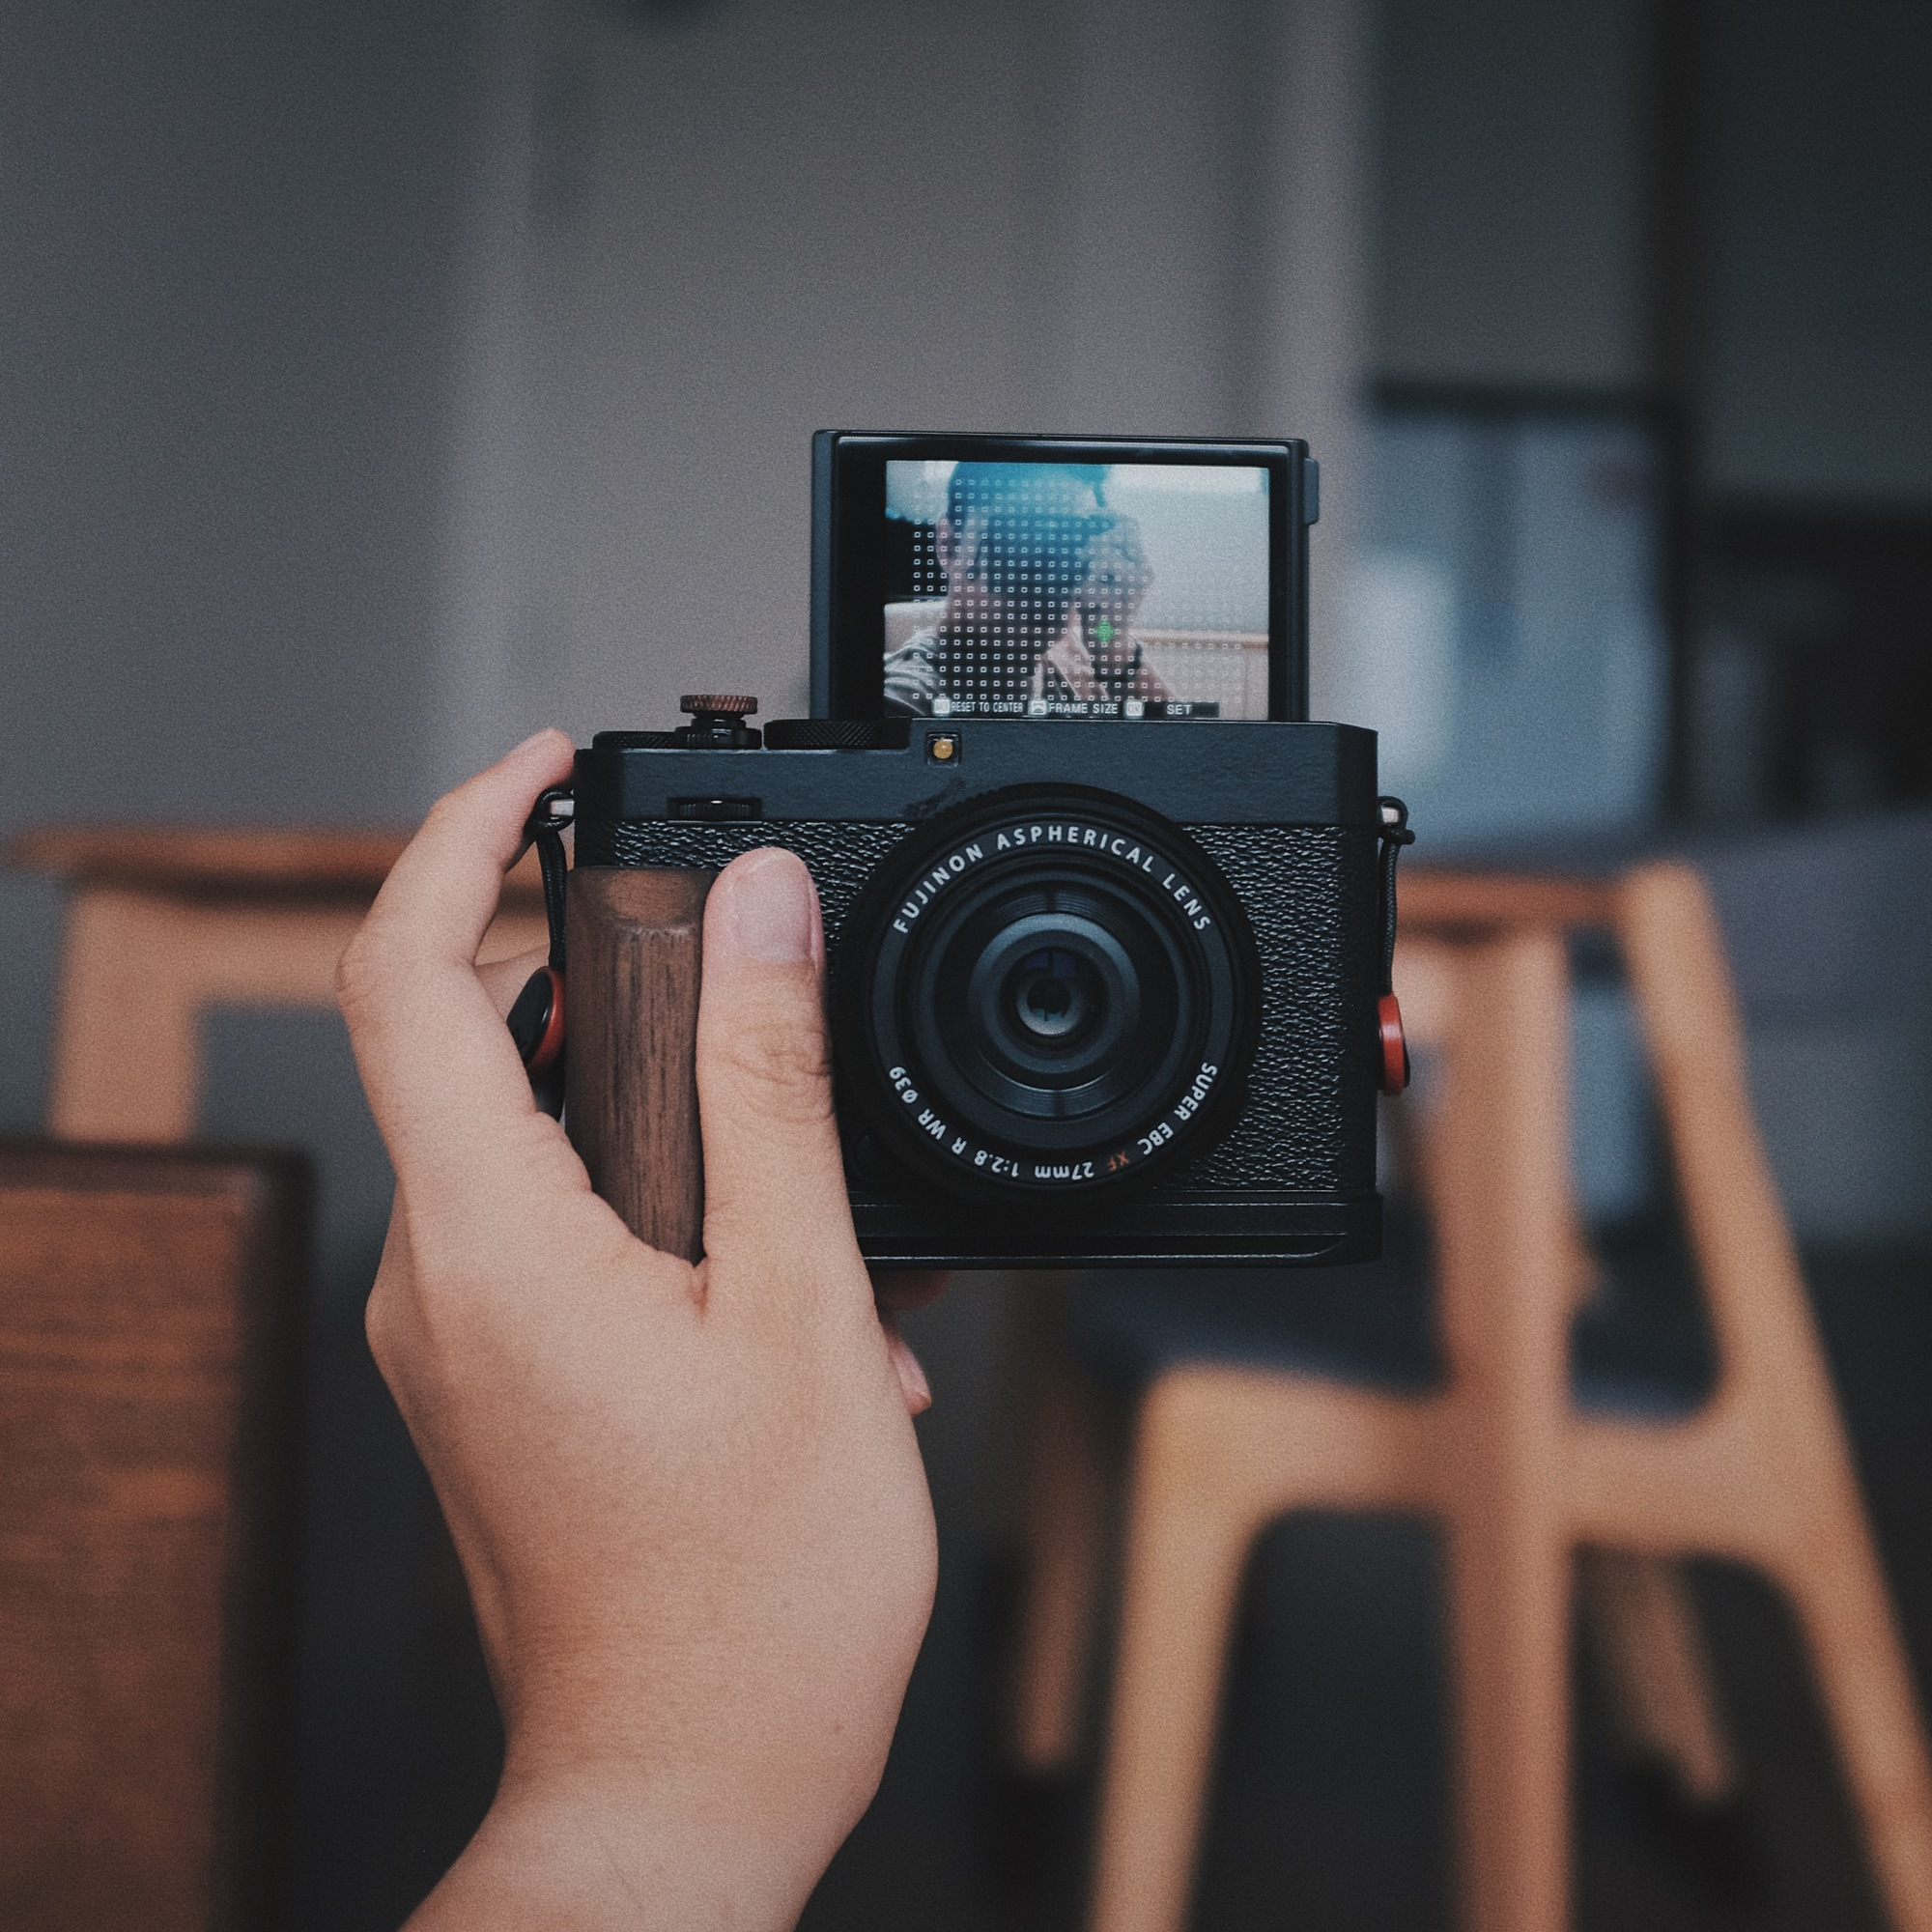
\includegraphics[width=\linewidth]{\envfinaldir/coverpic-prod.jpg}\par
            % \vskip 30pt
            \vfill

            \normalsize\rmfamily\scshape
            \copyright{} The Web Digest Project \hfill\large \envdatestr
        \end{center}
    \end{titlepage}
    % \restoregeometry
}
\newcommand{\simplehref}[1]{%
    \textcolor{blue!80!green}{\href{#1}{#1}}%
}
\renewcommand{\contentsname}{\center\Huge\sffamily\bfseries Contents\par\vskip 20pt}
\newcounter{ipartcounter}
\setcounter{ipartcounter}{0}
\newcommand{\ipart}[1]{
    % \vskip 20pt
    \clearpage
    \stepcounter{ipartcounter}
    \phantomsection
    \addcontentsline{toc}{chapter}{#1}
    % \begin{center}
    %     \Huge
    %     \sffamily\bfseries
    %     #1
    % \end{center}
    % \vskip 20pt plus 7pt
}
\newcounter{ichaptercounter}
\setcounter{ichaptercounter}{0}
\newcommand{\ichapter}[1]{
    % \vskip 20pt
    \clearpage
    \stepcounter{ichaptercounter}
    \phantomsection
    \addcontentsline{toc}{section}{\numberline{\arabic{ichaptercounter}}#1}
    \begin{center}
        \Huge
        \sffamily\bfseries
        #1
    \end{center}
    \vskip 20pt plus 7pt
}
\newcommand{\entrytitlefont}[1]{\subsection*{\raggedright\Large\sffamily\bfseries#1}}
\newcommand{\entryitemGeneric}[2]{
    % argv: title, url
    \parbox{\linewidth}{
        \entrytitlefont{#1}\par\vskip 5pt
        \footnotesize\ttfamily\mdseries
        \simplehref{#2}
    }\vskip 11pt plus 11pt minus 1pt
}
\newcommand{\entryitemGithub}[3]{
    % argv: title, url, desc
    \parbox{\linewidth}{
        \entrytitlefont{#1}\par\vskip 5pt
        \footnotesize\ttfamily\mdseries
        \simplehref{#2}\par\vskip 5pt
        \small\rmfamily\mdseries#3
    }\vskip 11pt plus 11pt minus 1pt
}
\newcommand{\entryitemAp}[3]{
    % argv: title, url, desc
    \parbox{\linewidth}{
        \entrytitlefont{#1}\par\vskip 5pt
        \footnotesize\ttfamily\mdseries
        \simplehref{#2}\par\vskip 5pt
        \small\rmfamily\mdseries#3
    }\vskip 11pt plus 11pt minus 1pt
}
\newcommand{\entryitemHackernews}[3]{
    % argv: title, hnurl, rawurl
    % \parbox{\linewidth}{
    %     \entrytitlefont{#1}\par\vskip 5pt
    %     \footnotesize\ttfamily\mdseries
    %     \simplehref{#3}\par
    %     \textcolor{black!50}{\href{#2}{#2}}
    % }\vskip 11pt plus 11pt minus 1pt
    \begin{minipage}{\linewidth}
            \entrytitlefont{#1}\par\vskip 5pt
            \footnotesize\ttfamily\mdseries
            \simplehref{#3}\par
            \textcolor{black!50}{\href{#2}{#2}}
    \end{minipage}\par\vskip 11pt plus 11pt minus 1pt
}







\begin{document}

\makeheader

\tableofcontents\clearpage




\ipart{Developers}
\ichapter{Hacker News}
\entryitemTwoLinks{I don't think AGI is right around the corner}{https://news.ycombinator.com/item?id=44483897}{https://www.dwarkesh.com/p/timelines-june-2025}

\entryitemTwoLinks{I extracted the safety filters from Apple Intelligence models}{https://news.ycombinator.com/item?id=44483485}{https://github.com/BlueFalconHD/apple\_generative\_model\_safety\_decrypted}

\entryitemTwoLinks{Show HN: I wrote a "web OS" based on the Apple Lisa's UI, with 1-bit graphics}{https://news.ycombinator.com/item?id=44482965}{https://alpha.lisagui.com/}

\entryitemTwoLinks{Opencode: AI coding agent, built for the terminal}{https://news.ycombinator.com/item?id=44482504}{https://github.com/sst/opencode}

\entryitemTwoLinks{Huawei cloned Qwen and DeepSeek models, claimed as own}{https://news.ycombinator.com/item?id=44482051}{https://dilemmaworks.substack.com/p/whistleblower-huawei-cloned-and-renamed}

\entryitemTwoLinks{Functions Are Vectors (2023)}{https://news.ycombinator.com/item?id=44481464}{https://thenumb.at/Functions-are-Vectors/}

\entryitemTwoLinks{Hannah Cairo: 17-year-old teen refutes a math conjecture proposed 40 years ago}{https://news.ycombinator.com/item?id=44481441}{https://english.elpais.com/science-tech/2025-07-01/a-17-year-old-teen-refutes-a-mathematical-conjecture-proposed-40-years-ago.html}

\entryitemTwoLinks{Building a Mac app with Claude code}{https://news.ycombinator.com/item?id=44481286}{https://www.indragie.com/blog/i-shipped-a-macos-app-built-entirely-by-claude-code}

\entryitemTwoLinks{Jane Street barred from Indian markets as regulator freezes \$566 million}{https://news.ycombinator.com/item?id=44480916}{https://www.cnbc.com/2025/07/04/indian-regulator-bars-us-trading-firm-jane-street-from-accessing-securities-market.html}

\entryitemTwoLinks{Stop killing games and the industry response}{https://news.ycombinator.com/item?id=44480284}{https://blog.kronis.dev/blog/stop-killing-games}

\entryitemTwoLinks{Get the location of the ISS using DNS}{https://news.ycombinator.com/item?id=44480223}{https://shkspr.mobi/blog/2025/07/get-the-location-of-the-iss-using-dns/}

\entryitemTwoLinks{MI5's falsehoods in the case of neo-Nazi spy who abused women}{https://news.ycombinator.com/item?id=44479029}{https://www.bbc.com/news/articles/c3w4nwdwywno}

\entryitemTwoLinks{The force-feeding of AI features on an unwilling public}{https://news.ycombinator.com/item?id=44478279}{https://www.honest-broker.com/p/the-force-feeding-of-ai-on-an-unwilling}

\entryitemTwoLinks{Are we the baddies?}{https://news.ycombinator.com/item?id=44478115}{https://geohot.github.io//blog/jekyll/update/2025/07/05/are-we-the-baddies.html}

\entryitemTwoLinks{Colombia seizes first unmanned narco-submarine with Starlink antenna}{https://news.ycombinator.com/item?id=44477601}{https://www.france24.com/en/americas/20250702-colombia-narco-submarine-starlink}

\entryitemTwoLinks{Volvo delivers 5,000th electric semi}{https://news.ycombinator.com/item?id=44477331}{https://electrek.co/2025/06/29/volvo-delivers-5000th-electric-semi-with-little-fanfare-sending-a-big-message/}

\entryitemTwoLinks{Serving 200M requests per day with a CGI-bin}{https://news.ycombinator.com/item?id=44476716}{https://simonwillison.net/2025/Jul/5/cgi-bin-performance/}

\entryitemTwoLinks{Hidden interface controls that affect usability}{https://news.ycombinator.com/item?id=44476297}{https://interactions.acm.org/archive/view/july-august-2025/stop-hiding-my-controls-hidden-interface-controls-are-affecting-usability}

\entryitemTwoLinks{What a Hacker Stole from Me}{https://news.ycombinator.com/item?id=44476115}{https://mynoise.net/blog.php}

\entryitemTwoLinks{Techno-feudalism and the rise of AGI: A future without economic rights?}{https://news.ycombinator.com/item?id=44475634}{https://arxiv.org/abs/2503.14283}


\ipart{Developers~~~~(zh-Hans)}
\ichapter{Solidot}
\entryitemGeneric{\hskip 0pt{}微软 XBox 业务高管建议被裁员的员工用 AI 管理情绪}{https://www.solidot.org/story?sid=81729}

\entryitemGeneric{\hskip 0pt{}美国面临其历史上最大规模的人才流失}{https://www.solidot.org/story?sid=81728}

\entryitemGeneric{\hskip 0pt{}善用表情符号能在交流中给对方留下好印象}{https://www.solidot.org/story?sid=81727}

\entryitemGeneric{\hskip 0pt{}《圣歌》服务器将于 2026 年 1 月关闭}{https://www.solidot.org/story?sid=81726}

\entryitemGeneric{\hskip 0pt{}云南甘棠箐遗址出土 30 万年前木质工具}{https://www.solidot.org/story?sid=81725}

\entryitemGeneric{\hskip 0pt{}科学家警告美国可能会失去一代人才}{https://www.solidot.org/story?sid=81724}

\entryitemGeneric{\hskip 0pt{}空气污染和传统草药与肺癌相关}{https://www.solidot.org/story?sid=81723}

\entryitemGeneric{\hskip 0pt{}挪威六月电动汽车占总销量的 96.9\% }{https://www.solidot.org/story?sid=81722}

\entryitemGeneric{\hskip 0pt{}Stop Killing Games 运动吸引了逾百万人签名}{https://www.solidot.org/story?sid=81721}

\entryitemGeneric{\hskip 0pt{}2024 年发表的医学论文摘要七分之一可能是 AI 完成的}{https://www.solidot.org/story?sid=81720}

\entryitemGeneric{\hskip 0pt{}Clothoff 试图支配深度伪造色情}{https://www.solidot.org/story?sid=81719}\ichapter{V2EX}
\entryitemGeneric{\hskip 0pt{}[酷工作] 谈一谈兼职朴朴超市骑手的感想}{https://www.v2ex.com/t/1143377}

\entryitemGeneric{\hskip 0pt{}[分享发现] 大家在 V2EX 特别关注了谁呢}{https://www.v2ex.com/t/1143375}

\entryitemGeneric{\hskip 0pt{}[问与答] 人生岔路口,工作方向选择,请各位前辈百忙之中指点一二}{https://www.v2ex.com/t/1143374}

\entryitemGeneric{\hskip 0pt{}[程序员] 分享一篇关于智能体的学习思考总结小文}{https://www.v2ex.com/t/1143373}

\entryitemGeneric{\hskip 0pt{}[分享发现] 关于情感反诈模拟器的游玩体验}{https://www.v2ex.com/t/1143371}

\entryitemGeneric{\hskip 0pt{}[分享发现] SEO 相关工具记录}{https://www.v2ex.com/t/1143370}

\entryitemGeneric{\hskip 0pt{}[宽带症候群] 为什么路由器上 mihomo 配置为 stack: system 时, WSL2 间歇性无法通过代理上网?}{https://www.v2ex.com/t/1143369}

\entryitemGeneric{\hskip 0pt{}[问与答] 诺亚内部人员关于华为盘古套壳千问的文章,大家怎么看?}{https://www.v2ex.com/t/1143368}

\entryitemGeneric{\hskip 0pt{}[OpenAI] Gemini Pro 能在 vscode 里面使用吗}{https://www.v2ex.com/t/1143366}

\entryitemGeneric{\hskip 0pt{}[推广] 一个新的土耳其虚拟卡}{https://www.v2ex.com/t/1143364}

\entryitemGeneric{\hskip 0pt{}[远程工作] (远程) 高性能 加速器 APP 开发}{https://www.v2ex.com/t/1143363}

\entryitemGeneric{\hskip 0pt{}[问与答] macos 升级到最新的系统 15.5 边框对不齐}{https://www.v2ex.com/t/1143362}

\entryitemGeneric{\hskip 0pt{}[问与答] 使用了 openclash 后如何修改 /etc/resolv.conf 文件}{https://www.v2ex.com/t/1143361}

\entryitemGeneric{\hskip 0pt{}[酷工作] 寻找一位能实现推荐功能的伙伴}{https://www.v2ex.com/t/1143360}

\entryitemGeneric{\hskip 0pt{}[职场话题] 小型企业老板,会在乎网络上对他的公司的评价吗?}{https://www.v2ex.com/t/1143358}

\entryitemGeneric{\hskip 0pt{}[分享发现] 分享一段和 ChatGPT 的对话,,,虽然我不认可这种 AI,但是它的回答还是挺好的。}{https://www.v2ex.com/t/1143356}

\entryitemGeneric{\hskip 0pt{}[Claude] Claude Code Pro 额度用完?脚本半夜自动续命!}{https://www.v2ex.com/t/1143355}

\entryitemGeneric{\hskip 0pt{}[VPS] racknerd 可靠吗?}{https://www.v2ex.com/t/1143354}

\entryitemGeneric{\hskip 0pt{}[Telegram] 大家有什么有意思的 telegram 群组或者频道}{https://www.v2ex.com/t/1143351}

\entryitemGeneric{\hskip 0pt{}[生活] 老婆买吃的喝的总是找这个券,那个券,总是把注意力放在这些事情上,我说她,她又生气,你们老婆也这样吗?想问问有什么好办法吗?}{https://www.v2ex.com/t/1143350}

\entryitemGeneric{\hskip 0pt{}[macOS] macos 如何让一个软件始终``置顶''显示}{https://www.v2ex.com/t/1143349}

\entryitemGeneric{\hskip 0pt{}[硬件] 辛苦各位 V 友帮忙看一下这个台式主机配置怎么样}{https://www.v2ex.com/t/1143347}

\entryitemGeneric{\hskip 0pt{}[OpenWrt] sing-box 裸核运行指南+批量机场节点导入配置模板教程(适用 windows/OpenWRT)}{https://www.v2ex.com/t/1143344}

\entryitemGeneric{\hskip 0pt{}[问与答] 上班之后如果想再出国读个硕士,随性一点的,有啥推荐么}{https://www.v2ex.com/t/1143343}

\entryitemGeneric{\hskip 0pt{}[程序员] 有哪些类似飞书多维表格的开源项目?}{https://www.v2ex.com/t/1143342}

\entryitemGeneric{\hskip 0pt{}[宽带症候群] 关于自建 RustDesk 远程被干掉 21116udp 端口这件事。}{https://www.v2ex.com/t/1143341}

\entryitemGeneric{\hskip 0pt{}[酷工作] 招聘: Product Manager 风控经理或总监 高级前端工程师(编译器方向)  Java 开发工程师 Marketing Associate(ZK-Content) Corporate Tax Manager}{https://www.v2ex.com/t/1143340}

\entryitemGeneric{\hskip 0pt{}[Windows] 24h2 真是垃圾啊,小问题一大堆}{https://www.v2ex.com/t/1143339}

\entryitemGeneric{\hskip 0pt{}[NAS] 天气太热,把 NAS 上机械硬盘摘下来了}{https://www.v2ex.com/t/1143338}

\entryitemGeneric{\hskip 0pt{}[Apple] APPLE 苹果产品参数中心 网站怎么没了呢? 还是改域名了?}{https://www.v2ex.com/t/1143337}

\entryitemGeneric{\hskip 0pt{}[职场话题] 准备二进宫回公司了,有什么要注意的嘛}{https://www.v2ex.com/t/1143336}

\entryitemGeneric{\hskip 0pt{}[酷工作] 招聘: AI 算法工程师 Flutter app Golang 工程师 测试工程师 前端工程师(Nodejs / React) DevOps 工程师 大数据开发工程师 低延迟量化交易开发工程师}{https://www.v2ex.com/t/1143335}

\entryitemGeneric{\hskip 0pt{}[问与答] 深圳有哪些适合一个人的好去处?或者在家能做哪些事?}{https://www.v2ex.com/t/1143332}

\entryitemGeneric{\hskip 0pt{}[摄影] 在济西国家湿地公园拍到了``温度计''}{https://www.v2ex.com/t/1143331}

\entryitemGeneric{\hskip 0pt{}[创业组队] 有开发运营过 Shopify App 的朋友,项目合作}{https://www.v2ex.com/t/1143330}

\entryitemGeneric{\hskip 0pt{}[Go 编程语言] 为什么这段代码能够顺序的打印出 1-10,没太理解?}{https://www.v2ex.com/t/1143329}

\entryitemGeneric{\hskip 0pt{}[问与答] 国内有类 Flic Button 的产品吗?}{https://www.v2ex.com/t/1143328}

\entryitemGeneric{\hskip 0pt{}[Cursor] Cursor 与 Claude Code: AI 编程助手深度对比}{https://www.v2ex.com/t/1143327}

\entryitemGeneric{\hskip 0pt{}[问与答] 为啥微信语音消息不能转发呢?是技术原因吗}{https://www.v2ex.com/t/1143325}

\entryitemGeneric{\hskip 0pt{}[程序员] 感觉我的 bun 安装依赖越来越慢了,有大佬知道什么原因吗}{https://www.v2ex.com/t/1143324}

\entryitemGeneric{\hskip 0pt{}[分享创造] 新做的小工具 软著登记申请文件自动生成 免费使用}{https://www.v2ex.com/t/1143323}

\entryitemGeneric{\hskip 0pt{}[推广] 我的开源项目,官网域名好像被墙了}{https://www.v2ex.com/t/1143322}

\entryitemGeneric{\hskip 0pt{}[问与答] 请问哪款电动窗帘可以接入 home assistant ?}{https://www.v2ex.com/t/1143321}

\entryitemGeneric{\hskip 0pt{}[分享发现] 芬兰 CS 硕士毕业,顺利找到工作}{https://www.v2ex.com/t/1143320}

\entryitemGeneric{\hskip 0pt{}[问与答] aria2 在 Flutter 应用中卡住的原因及解决方案?}{https://www.v2ex.com/t/1143319}

\entryitemGeneric{\hskip 0pt{}[硬件] [请教]可更换电池的充电宝,是不是最优解?}{https://www.v2ex.com/t/1143318}

\entryitemGeneric{\hskip 0pt{}[Apple] 外区的 B 站 APP 未来不更新了,国区的 B 站 APP 有啥去广告以后不影响正常使用的规则吗}{https://www.v2ex.com/t/1143317}

\entryitemGeneric{\hskip 0pt{}[问与答] 海康威视的云存储}{https://www.v2ex.com/t/1143316}

\entryitemGeneric{\hskip 0pt{}[宽带症候群] 广东联通高峰期丢包}{https://www.v2ex.com/t/1143315}

\entryitemGeneric{\hskip 0pt{}[VXNA] 申请收录个人博客: voxsay.com}{https://www.v2ex.com/t/1143312}


\ipart{Generic News}







\clearpage
\leavevmode\vfill
\footnotesize

Copyright \copyright{} 2023-2025 Neruthes and other contributors.

This document is published with CC BY-NC-ND 4.0 license.

The entries listed in this newsletter may be copyrighted by their respective creators.

This newsletter is generated by the Web Digest project.

The newsletters are also delivered via Telegram channel \CJKunderline{\href{https://t.me/webdigestchannel}{https://t.me/webdigestchannel}}.\\
RSS feed is available at \CJKunderline{\href{https://webdigest.pages.dev/rss.xml}{https://webdigest.pages.dev/rss.xml}}.

This newsletter is available in PDF at
\CJKunderline{\href{https://webdigest.pages.dev/}{https://webdigest.pages.dev/}}.

The source code being used to generate this newsletter is available at\\
\CJKunderline{\href{https://github.com/neruthes/webdigest}{https://github.com/neruthes/webdigest}}.

This newsletter is also available in
\CJKunderline{\href{http://webdigest.pages.dev/readhtml/\envyear/WebDigest-20250707.html}{HTML}} and
\CJKunderline{\href{https://github.com/neruthes/webdigest/blob/master/markdown/\envyear/WebDigest-20250707.md}{Markdown}}.


\coverpic{https://unsplash.com/photos/woman-stands-on-beach-reflecting-at-sunset-NC5ZsT7tHWQ}{Karsten Winegeart}


\end{document}
